Unlike the experiment, the Monte Carlo simulation allows one to exclude
certain events from ever being generated.  In this case, it is
important to note that these trajectories aren't removed from the
simulation - rather they are never generated in the first place.
Therefore, if you run a simulation specifying $N$ events, the result will
be $N$ events of only the type allowed.  

Though any arbitrary event can be excluded from the simulation, we are
categorically interested in four main types (Figure \ref{fig:scattypes}).
They are
\begin{enumerate}[I]
\item Single scattering involving the tip - a trajectory including only the
tip.
\item Single scattering {\bf NOT} involving the tip - a trajectory including only
one scatterer which is not the tip.
\item Multiple scattering involving the tip - a trajectory including two or
more scatterers where at least one of them is the tip.
\item Multiple scattering {\bf NOT} involving the tip - a trajectory including
more than one scatterer where \underline{none} of those scatterers is the tip.
\end{enumerate}
\begin{figure}
\centering
\subfigure[single scattering including tip]{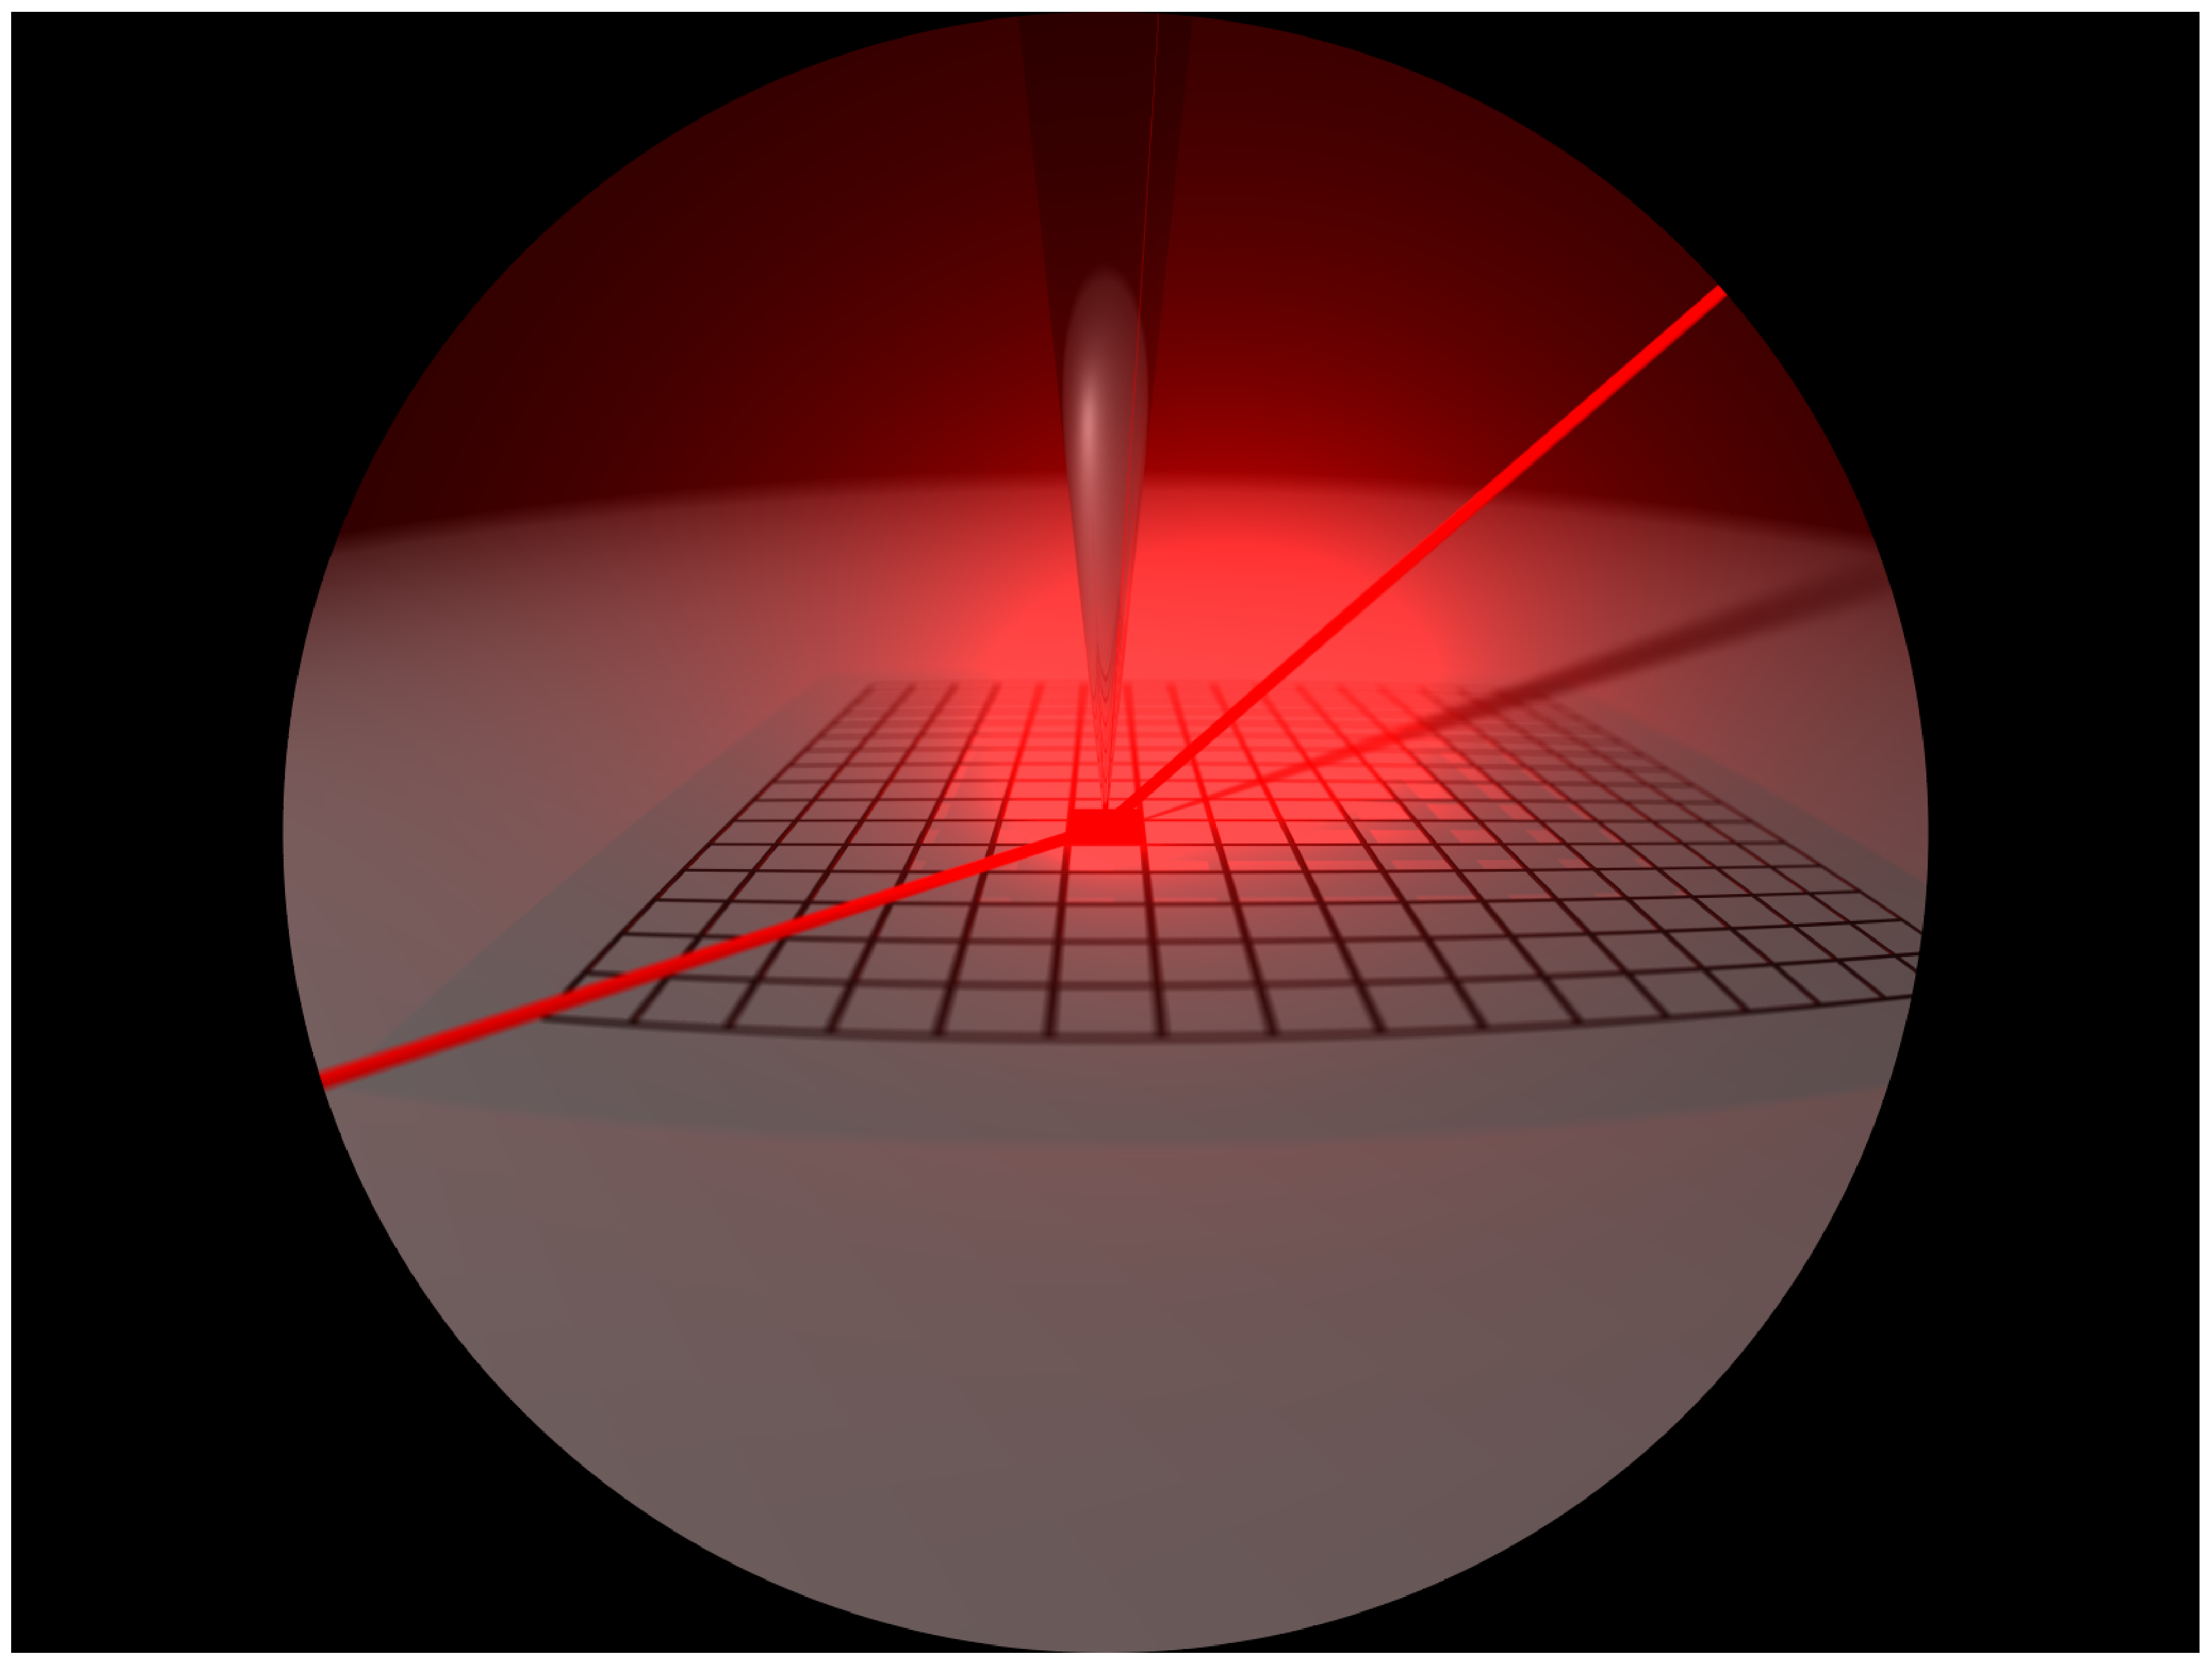
\includegraphics[width=5cm]{simulation/singlescatt.eps}}
\subfigure[single scattering not including tip]{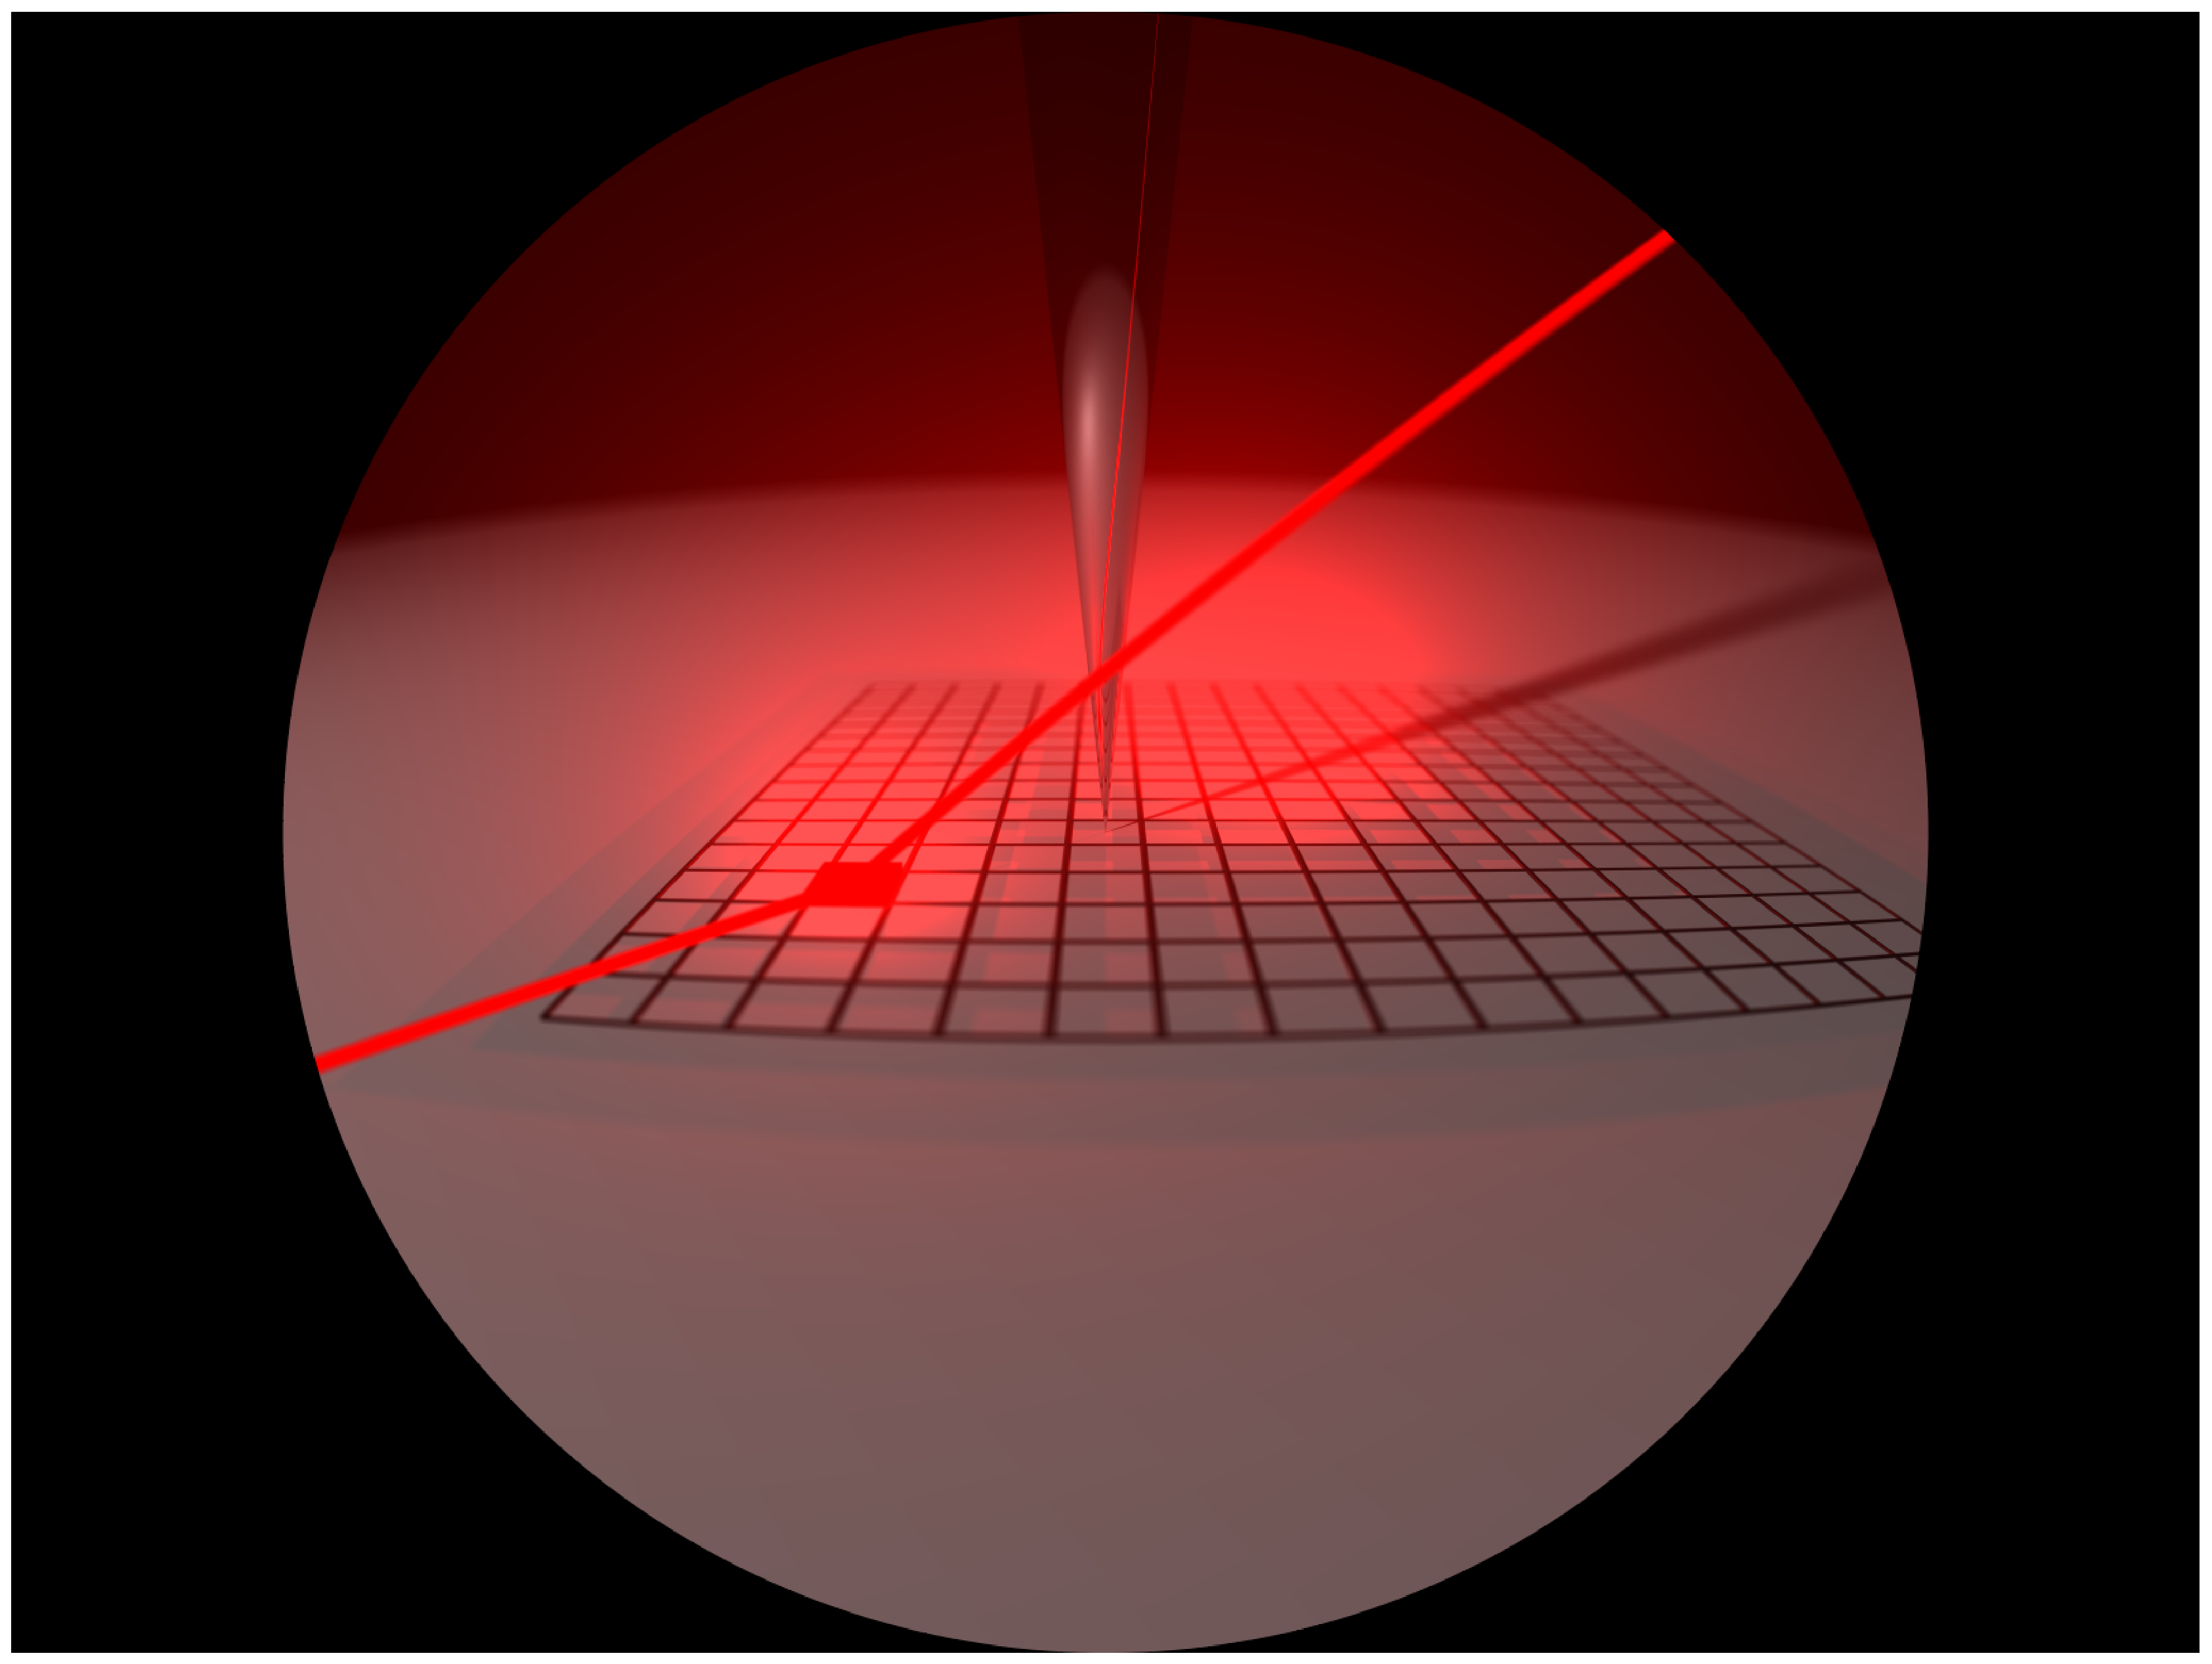
\includegraphics[width=5cm]{simulation/singlescattnotpip.eps}}\\
\subfigure[multiple scattering including tip]{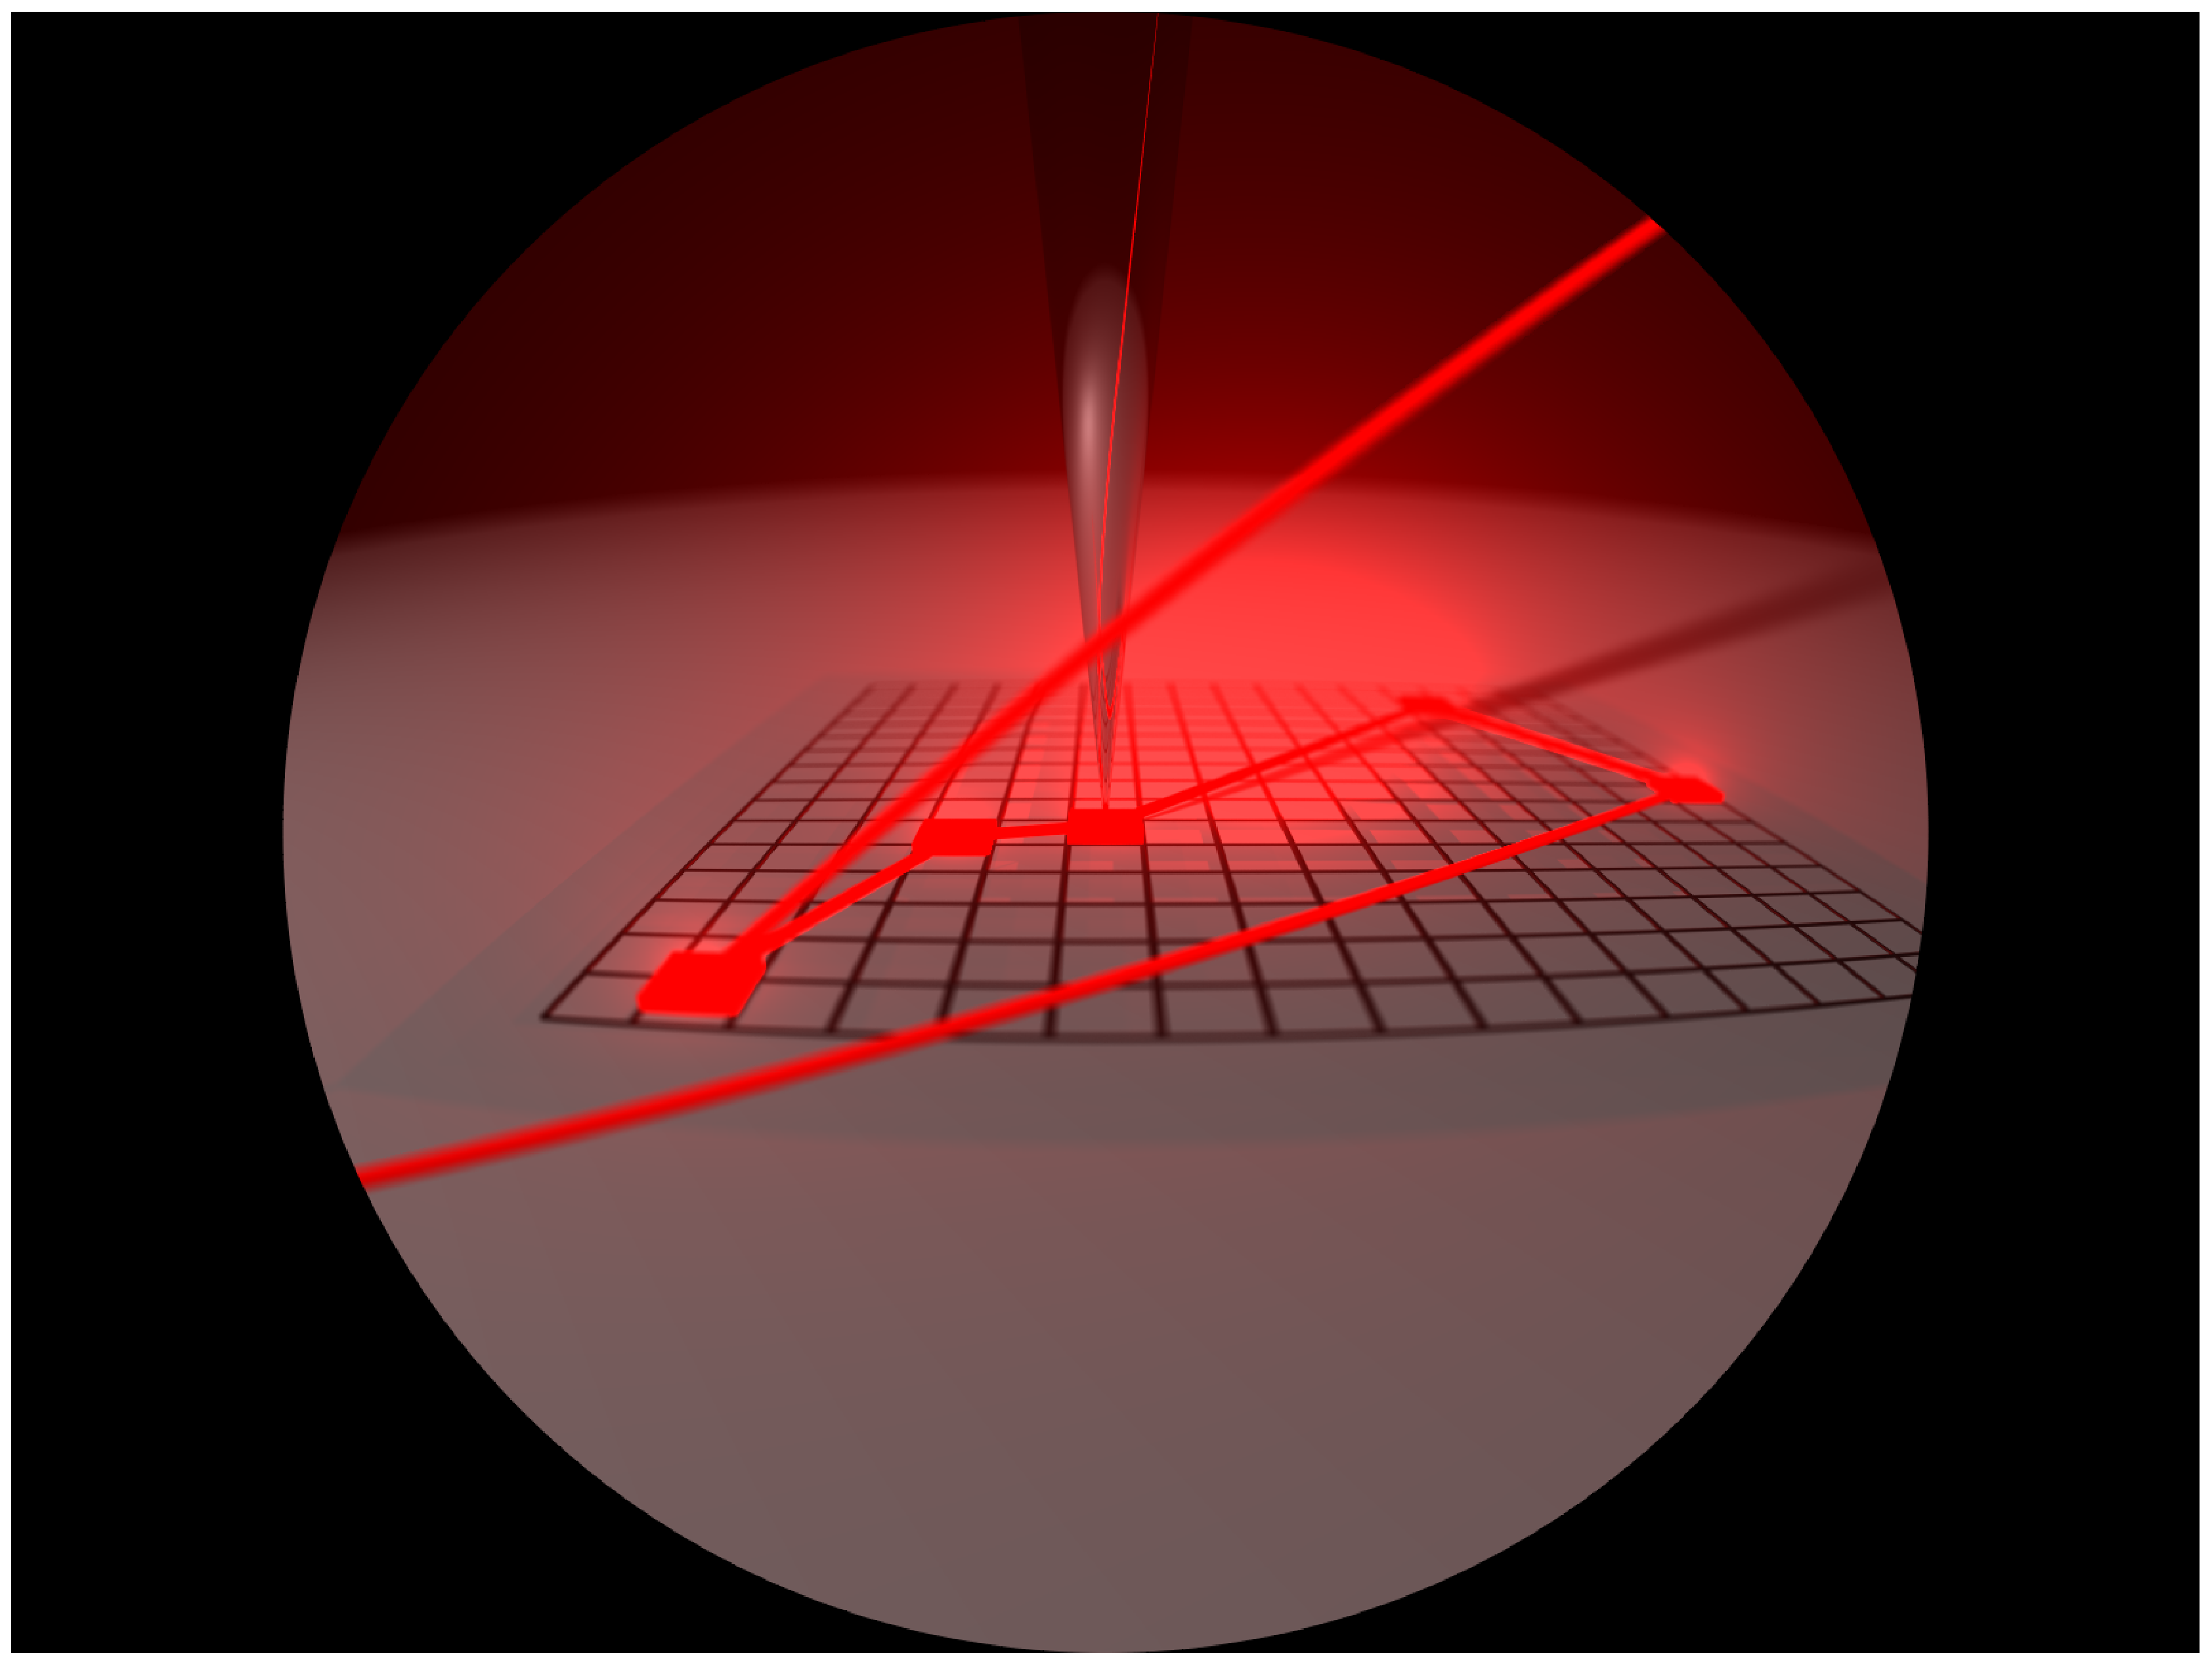
\includegraphics[width=5cm]{simulation/multiplescatt.eps}}
\subfigure[multiple scattering not including tip]{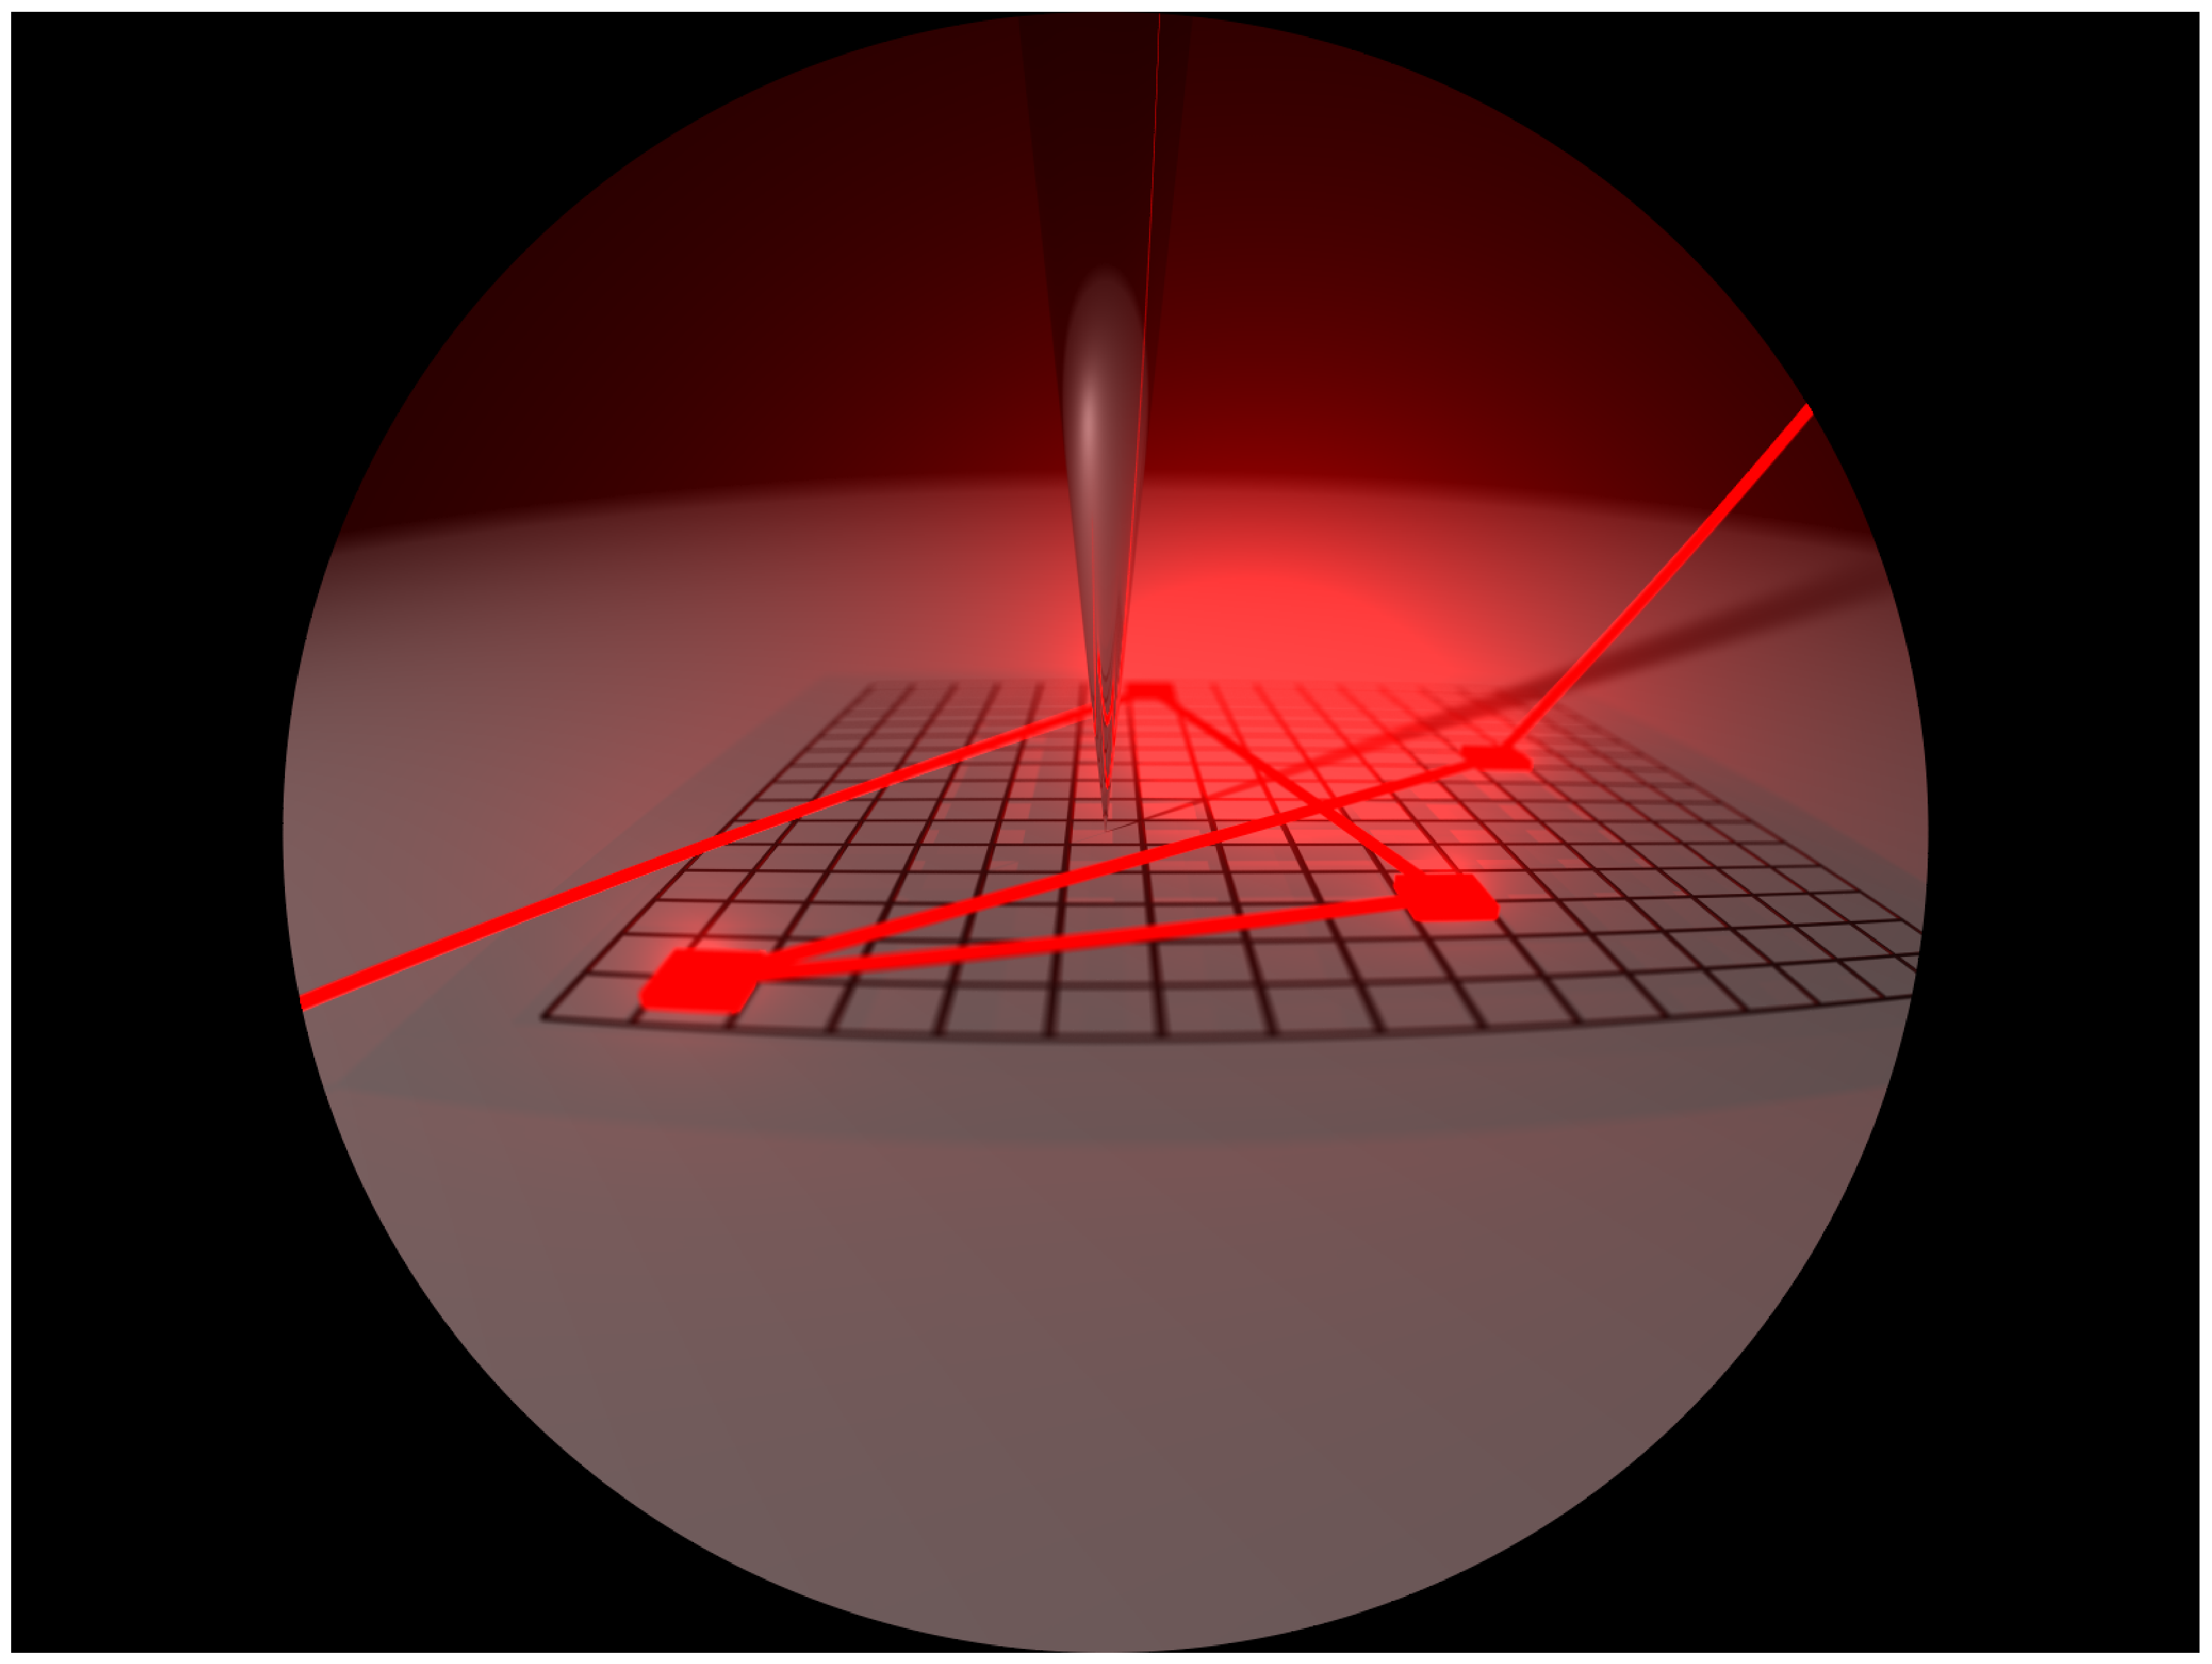
\includegraphics[width=5cm]{simulation/multiplescattnotip.eps}}
\caption{Types of scattering events we include or exclude from the simulation.}
\label{fig:scattypes}
\end{figure}

If we treat each of the four event types as a binary number ($1=$ included
in the simulation, $0=$ excluded from the simulation), there are $2^4=16$
distinct possibilities among them.  To this accord, and in the figures to
follow, they are arranged with the convention in Figure
\ref{fig:cleverbinary}.  In each cell, the color gray represents the type of
scattering event which has been excluded.
\begin{figure}
\centering
\psscalebox{0.7}{
\psset{unit=1.1cm}
  \begin{pspicture}(0,0)(6,6)
  \psframe[fillcolor=gray,fillstyle=solid](-1.5,0)(0,1.5)
  \psframe[fillcolor=gray,fillstyle=solid](-1.5,1.5)(0,3)
  \psframe[fillcolor=gray,fillstyle=solid](-1.5,3)(0,4.5)
  \psframe[fillcolor=gray,fillstyle=solid](-1.5,4.5)(0,6)
  \rput[c](-0.75,0.75){\Rmnum{4}}
  \rput[c](-0.75,2.25){\Rmnum{3}}
  \rput[c](-0.75,3.75){\Rmnum{2}}
  \rput[c](-0.75,5.25){\Rmnum{1}}

  \psframe[](0,0)(6,1.5)
  \psframe[](0,1.5)(6,3)
  \psframe[](0,3)(6,4.5)
  \psframe[](0,4.5)(6,6)
  \rput[c](3,5.25){{single scattering involving the tip}}
  \rput[c](3,3.75){{single scattering not involving the tip}}
  \rput[c](3,2.25){{multiple scattering involving the tip}}
  \rput[c](3,0.75){{multiple scattering not involving the tip}}
  \end{pspicture}
}
\caption{The figures to follow have an accompanying sequence of four
vertical squares.  These squares represent which events have been excluded 
from the simulation.  Squares in {\gray gray} represent excluded events.}
\label{fig:cleverbinary}
\end{figure}
